\documentclass[a4paper]{article}
\usepackage[utf8]{inputenc}
\usepackage[english]{babel}
\usepackage{amsmath} % per ambienti tipo cases
\usepackage{amssymb}
\usepackage{mathtools}
\usepackage{siunitx}
\usepackage{graphicx} % per includere figure
%\usepackage{subfigure}
\usepackage{wrapfig}
\usepackage{booktabs} % per le tabelle
\usepackage{caption}
\usepackage{fancyhdr}
\usepackage{hyperref}
\usepackage[section]{placeins}
\usepackage{microtype}
\usepackage{caption}
\usepackage{subcaption}
\usepackage{listings}
\usepackage{xcolor}
%\captionsetup[subfigure]{labelfont=rm}
\usepackage{verbatim} %multiline comments
%\usepackage[backend=biber, style=numeric, safeinputenc, sorting=none]{biblatex}
%\addbibresource{source.bib}	% uncomment for bibliography

\definecolor{codegreen}{rgb}{0,0.6,0}
\definecolor{codegray}{rgb}{0.5,0.5,0.5}
\definecolor{codepurple}{rgb}{0.58,0,0.82}
\definecolor{backcolour}{rgb}{0.95,0.95,0.92}

\lstdefinestyle{mystyle}{
	backgroundcolor=\color{backcolour},   
	commentstyle=\color{codegreen},
	keywordstyle=\color{magenta},
	numberstyle=\tiny\color{codegray},
	stringstyle=\color{codepurple},
	basicstyle=\ttfamily\footnotesize,
	breakatwhitespace=false,         
	breaklines=true,                 
	captionpos=b,                    
	keepspaces=true,                 
	numbers=left,                    
	numbersep=5pt,                  
	showspaces=false,                
	showstringspaces=false,
	showtabs=false,                  
	tabsize=2
}

\lstset{style=mystyle}

%opening
\title{}
\author{}

\pagestyle{fancy}
\lhead{Musical Acoustics}
\chead{HL4}
\rhead{10743504, 10751919}
\newcommand{\Rarrow}{\mbox{\Large$\Rightarrow$}}

\begin{document}

\begin{titlepage}	
	\newcommand{\HRule}{\rule{\linewidth}{0.5mm}} % Defines a new command for horizontal lines, change thickness here
	
	\center % Centre everything on the page
	
	%------------------------------------------------
	%	Headings
	%------------------------------------------------
	
	
\includegraphics[width=.4\textwidth]{Logo_Politecnico_Milano.png}\\[0.4cm]
	\textsc{\LARGE}\\[0.3cm] % Main heading such as the name of your university/college
	
	\textsc{\large MSc. Music and Acoustic Engineering}\\[1cm] % Minor heading such as course title
	
	\textsc{\Large Musical Acoustics - A.Y. 2020/2021}\\[0.5cm] % Major heading such as course name
	
	%------------------------------------------------
	%	Title
	%------------------------------------------------
	
	\HRule\\[0.4cm]
	
	{\huge\bfseries HL4 – Radiance Estimation}\\[0.4cm] % Title of your document
	
	\HRule\\[1.5cm]
	
	
	
	{\large\textit{Authors' IDs:}}\\
	10743504, 10751919, % Your name
	%\\ \textsc{Gruppo 11}
	
	%------------------------------------------------
	%	Date
	%------------------------------------------------
	
	\vfill\vfill\vfill % Position the date 3/4 down the remaining page
	
	{\large\today} % Date, change the \today to a set date if you want to be precise
	
	%------------------------------------------------
	%	Logo
	%------------------------------------------------
	
	\vfill\vfill
	%\includegraphics[width=0.2\textwidth]{Politecnico_di_Milano.eps}\\[1cm] % Include a department/university logo - this will require the graphicx package
	
	%----------------------------------------------------------------------------------------
	
	\vfill % Push the date up 1/4 of the remaining page
	
	
\end{titlepage}

\section{Signal observation}
\begin{figure}[h]
	\centering
	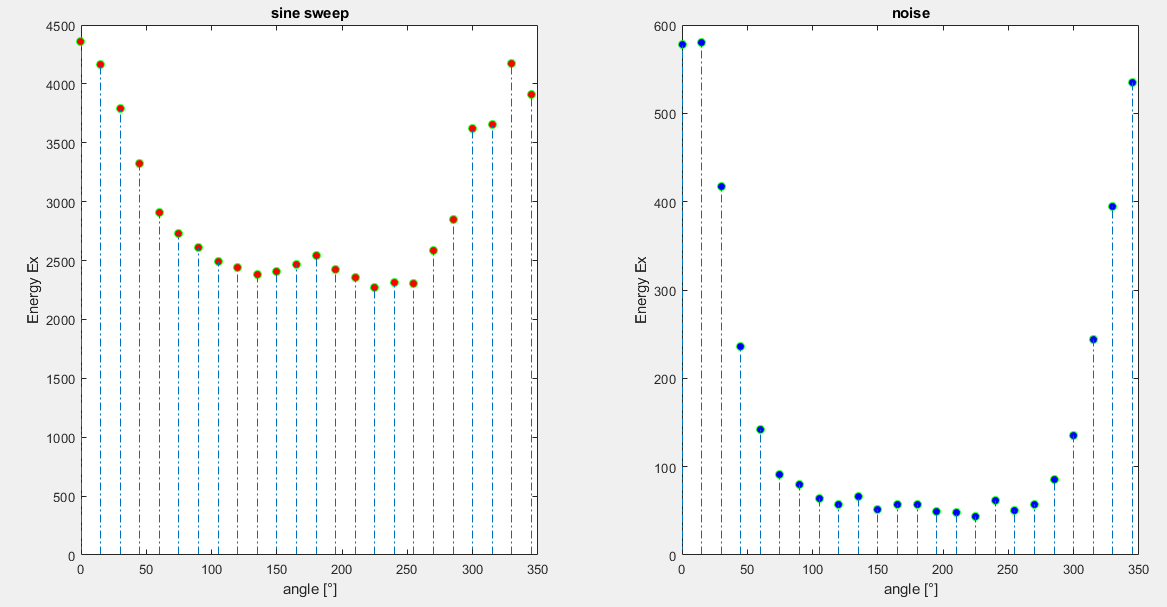
\includegraphics[width=0.75\linewidth]{sig_energy.png}
	\caption{Energies of the recorded signals as functions of the angle of acquisition.}
	\label{fig:energy}
\end{figure}

In \verb|exercise1.m| we label the signals with the angle at which they were recorded and the related type of input. We then compute the energies of the signals with the function\footnote{This function has been added to the provided \texttt{Functions} folder.} shown in List. \ref{list:nrg}. The energies of the sine sweep signals are larger than those of the noise signals, which is expected since the sweep acquisitions were longer (10 vs. 3 seconds). Either way, Fig. \ref{fig:energy} shows that the dependency on the angle is similar, as the energies are larger the closer we are to having the speaker pointed directly towards the microphone. Other specifics of the implementation, in this as in the other exercises, are explained in the comments of the Matlab scripts.

\begin{lstlisting}[language=Matlab, caption=compute\_energy.m, label=list:nrg]
	function [energy] = compute_energy(input)
		len = length(input);
		energy = 0;
		
		for i = 1:len
		energy = energy + abs(input(i))^2;
		end
	
	end
\end{lstlisting}

\section{Room reflection analysis using autocorrelation}
\begin{table}[h!]
	\centering
	$\begin{array}{l|ccc}
		\toprule
		& \text{\textbf{sweep}} & \text{\textbf{noise}} & \text{\textbf{both}}\\
		\hline
		\text{TOA\textsubscript{r} [ms]} & 3.00 \pm 0.05 & 3.20 \pm 0.06 & 3.1 \pm  0.1 \\
		r\text{ [m]} & 1.03 \pm 0.02 & 1.10 \pm 0.02 & 1.07 \pm 0.03\\
		\bottomrule
	\end{array}$
	\caption{Estimated time of arrival of the first reflection and microphone-reflector distance. From left to right, the averages over the sweep signals, the noise signals and over the entire set.}
	\label{tab:refl}
\end{table}

\begin{figure}[h]
	\centering
	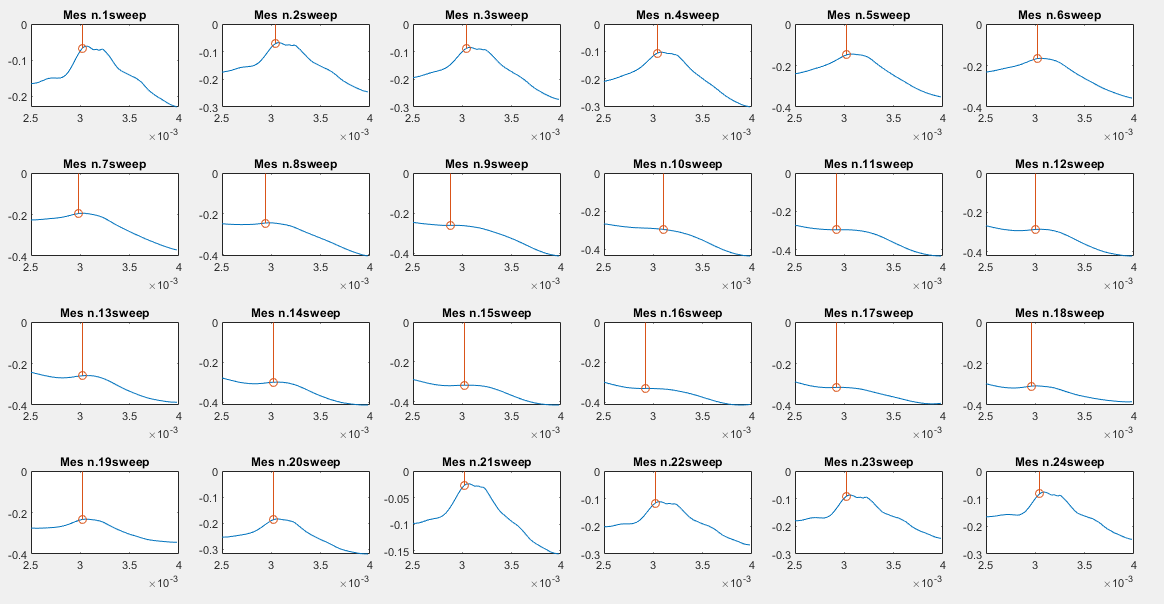
\includegraphics[width=0.85\linewidth]{sweep_peaks.png}
	\caption{First peaks of the autocorrelation functions for the \textbf{sweep signals}. A small portion of the autocorrelation is shown and the stem highlights the position of the peak.}
	\label{fig:sweepcorr}
\end{figure}

\begin{figure}[h]
	\centering
	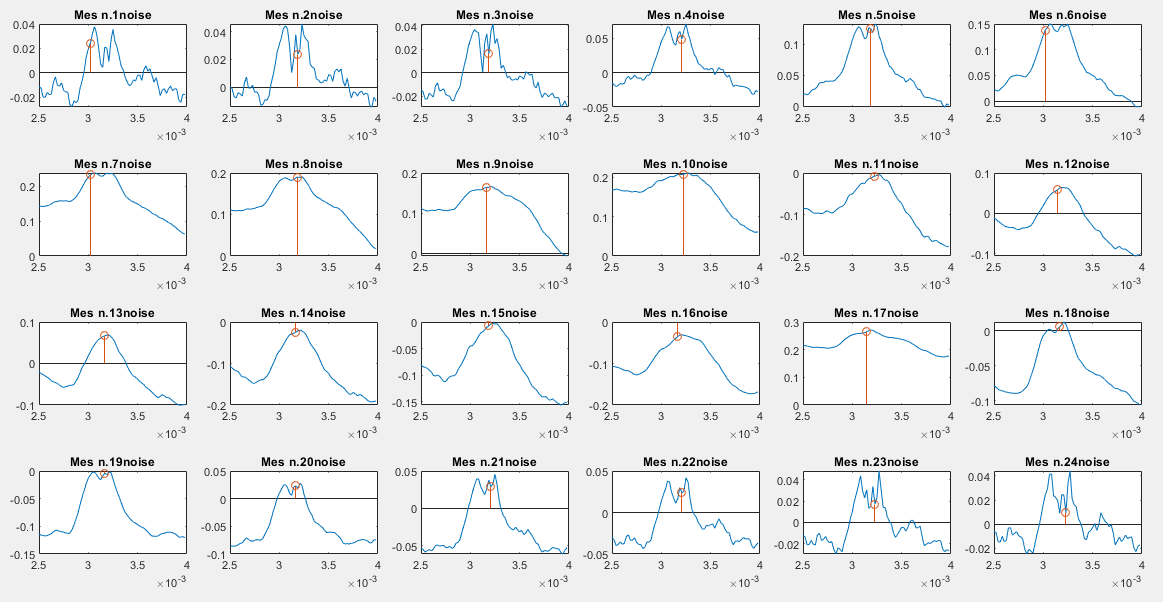
\includegraphics[width=0.85\linewidth]{noise_peaks.png}
	\caption{First peaks of the autocorrelation functions for the \textbf{noise signals}. A small portion of the autocorrelation is shown and the stem highlights the position of the peak.}
	\label{fig:noisecorr}
\end{figure}


In \verb|exercise2.m| we estimate the first reflection time from the autocorrelation of the recorded signals. The autocorrelation is computed and then visualized in order to find the first reflection; a small portion ($\sim$ 2 ms) of the signal around the selected peak is then extracted and the library function \verb|findpeaks| is run on it in order to estimate the exact location of the peak (see Figs. \ref{fig:sweepcorr} and \ref{fig:noisecorr}).

We then find an estimate of the time of arrival of the first reflection by taking the average and standard deviation of the locations of the peaks.  We can use this value to compute the distance of the microphone from the reflector by multiplying them for the speed of sound $c$. The results are reported in Tab. \ref{tab:refl}. As we can see, both methods yield similar results with comparable precision. However, we can see that, comparing it to the  sweep autocorrelations, the noise autocorrelations exhibit more high-frequency noise, which makes the estimation of the peak position slighlty less precise, especially close to 0°. On the other hand, though, if we zoom out (Fig. \ref{fig:autocorr}), we can see that the sweep autocorrelations are far noisier overall, due to the periodicity of the input signal, and this makes locating the first peak by visual inspection significantly harder, to the point that, without having the TOA estimated from the noise signals as a reference, it would be hard to tell whether the peak we are choosing is the correct one or merely an artifact. Overall, this leads us to conclude that measurements with the noise source are more reliable.


\begin{figure}
	\centering
	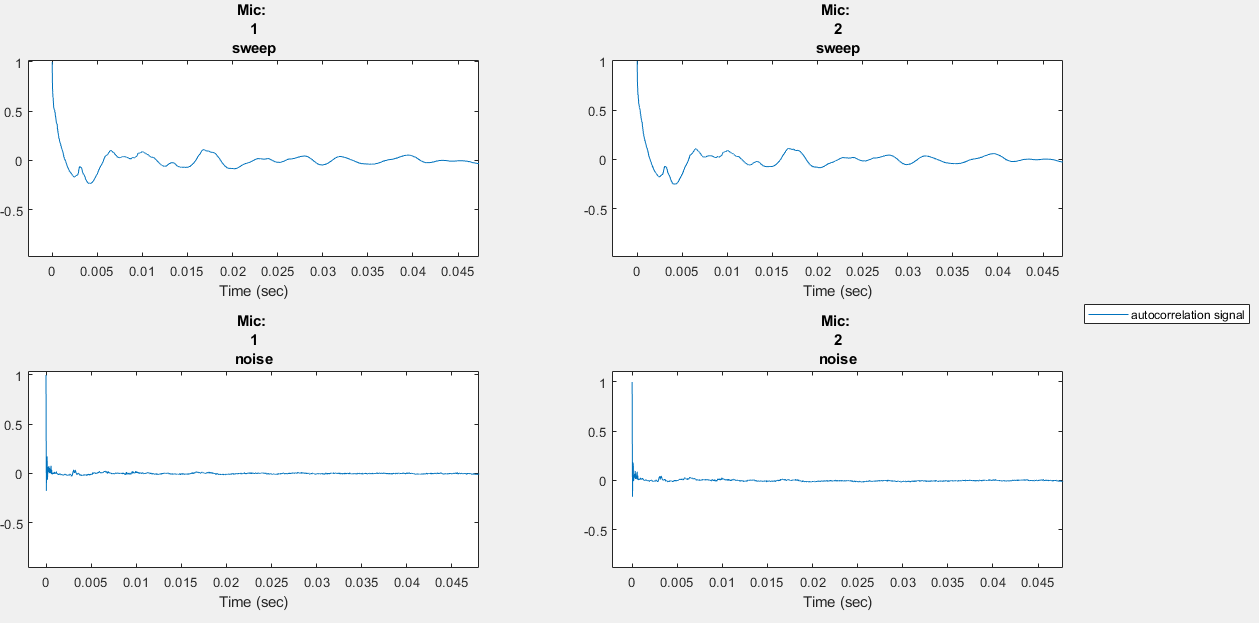
\includegraphics[width=0.75\linewidth]{autocorrelation.png}
	\caption{Autocorrelation for two sweep signals and two noise signals fro 0 to 45 ms.}
	\label{fig:autocorr}
\end{figure}

\section{Room reflection analysis using impulse responses}

\begin{table}[h!]
	\centering
	$\begin{array}{l|cc}
		\toprule
		& \text{\textbf{sweep}} & \text{\textbf{noise}} \\
		\hline
		\text{TOA\textsubscript{dir} [ms]} & 8.0 \pm 0.2 & 8.0 \pm 0.2\\
		\text{TOA\textsubscript{r} [ms]} & 3.22 \pm 0.06  & 3.2 \pm 0.1\\
		R \text{ [m]} & 1.12 \pm 0.02 & 1.11 \pm 0.04 \\
		\bottomrule
	\end{array}$
	\caption{Average values of the time of arrival of the direct signal, of the delay of the first reflection and of the source-microphone distance. }
	\label{tab:ir}
\end{table}

Here we wrote two scripts, one for the noise source (\verb|exercise3a.m|) and one for the sine sweep (\verb|exercise3b.m|). The aim is to compute the impulse responses from each measurement and use it to infer the TOAs of the direct signal and of the first reflection. The IRs can be obtained by dividing the FFT of the recorded signal by the FFT of the input and then taking the IFFT. We expect to find two major peaks at the beginning of the IRs, the first one corresponding to the direct signal and the second one corresponding to the first reflection. These peaks are first found visually like in the previous section, and then located with \verb|findpeaks| (see Figs. \ref{fig:noiseir} and \ref{fig:sweepir}).

The values of the direct TOAs obtained in this way are multiplied by $c$ to obtain the distance of the microphone from the source. These values are reported in Fig. \ref{fig:distance}.  It can be seen how the values obtained with the two methods look very similar, and how the estimation of the distance increases as the speaker points further away from the microphone and it decreases again as the orientation circles back to the full 360° angle. In Tab. \ref{tab:ir} we report also the average values of the direct TOA, of the first reflection delay and of the distance between the source and the microphone. Notice that the value of the delay is compatible with the one estimated from the autocorrelation in the case of the noise signals, while the ones for the sweep signal are within $\sim 3\sigma $ of eachother.

\begin{figure}[h]
	\centering
	\begin{subfigure}{0.47\linewidth}
		\centering
		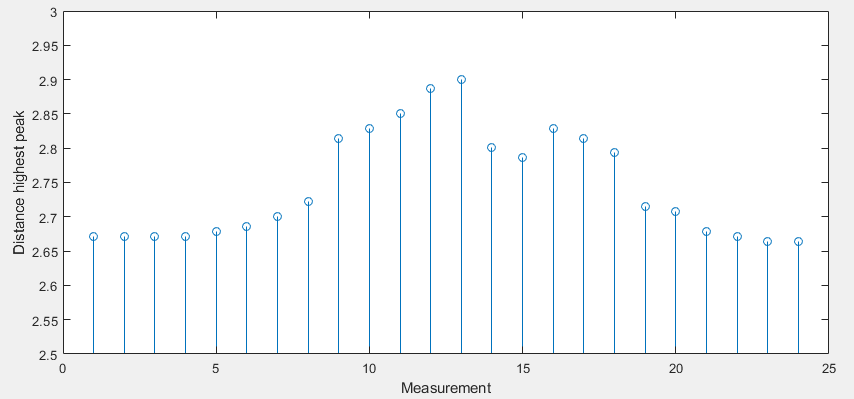
\includegraphics[width=0.9\linewidth]{noise_distance.png}
	\end{subfigure}
	~
	\begin{subfigure}{0.47\linewidth}
		\centering
		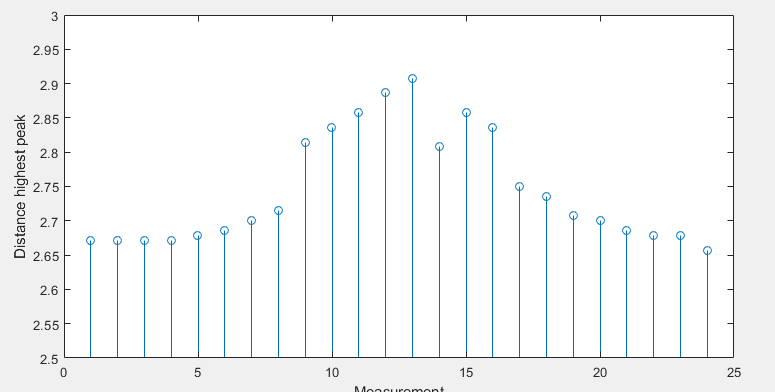
\includegraphics[width=0.9\linewidth]{sweep_distance.png}
	\end{subfigure}
	\caption{Estimated distance from the source as a function of the angle. On the left the estimates obtained with the noise input, while on the right those obtained with the sine sweep input.}
	\label{fig:distance}
\end{figure}



\begin{figure}[h]
	\centering
	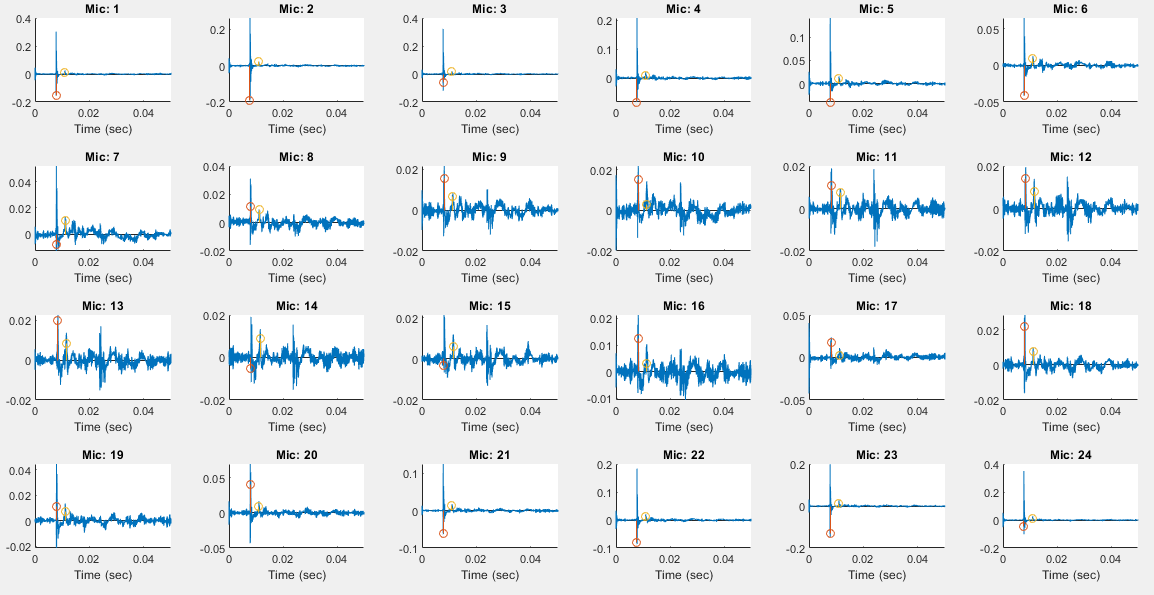
\includegraphics[width=0.85\linewidth]{noise_ir.png}
	\caption{Impulse responses for the \textbf{noise signals}. The stems highlight the direct and first reflection TOAs.}
	\label{fig:noiseir}
\end{figure}

\begin{figure}[h]
	\centering
	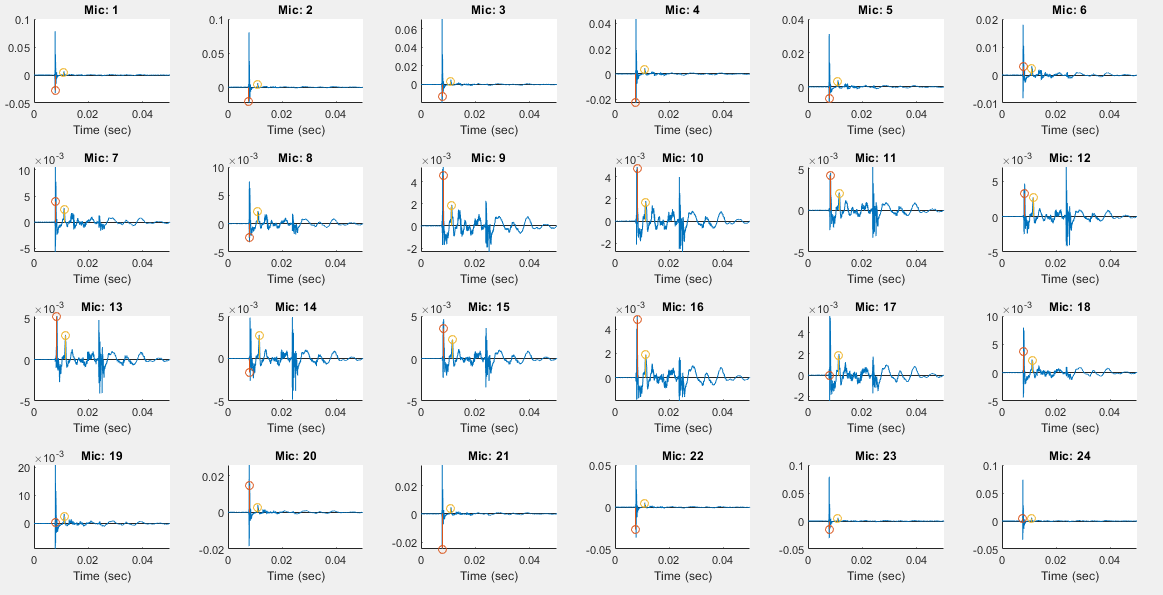
\includegraphics[width=0.85\linewidth]{sweep_ir.png}
	\caption{Impulse responses for the \textbf{sweep signals}. The stems highlight the direct and first reflection TOAs.}
	\label{fig:sweepir}
\end{figure}


\section{Radiance estimation directly from the signals}
The scripts for this section are \verb|exercise4a.m| (noise) and \verb|exercise4b.m| (sweep). We want to estimate the radiance pattern of the source: to do so, we window the recorded signal so that it only includes the direct sound. Then we can use the windowed signal to compute the impulse response of the free field (anechoic), which, knowing the distance $R$ from the source, can be used to derive the directivity function, i. e. the radiation pattern's absolute value.

We begin from the noise signals. We performed these operations using a Hanning window centered at the previously computed direct TOA. The suggested value for the length of the window (701 samples = 14.6 ms) leaves the first reflection inside; therefore we tried a shorter window as well (241 samples = 5 ms). The resulting radiance plots can be seen in Fig. \ref{fig:noiserad4}.

\begin{figure}[h]
	\centering
	\begin{subfigure}{0.85\linewidth}
		\centering
		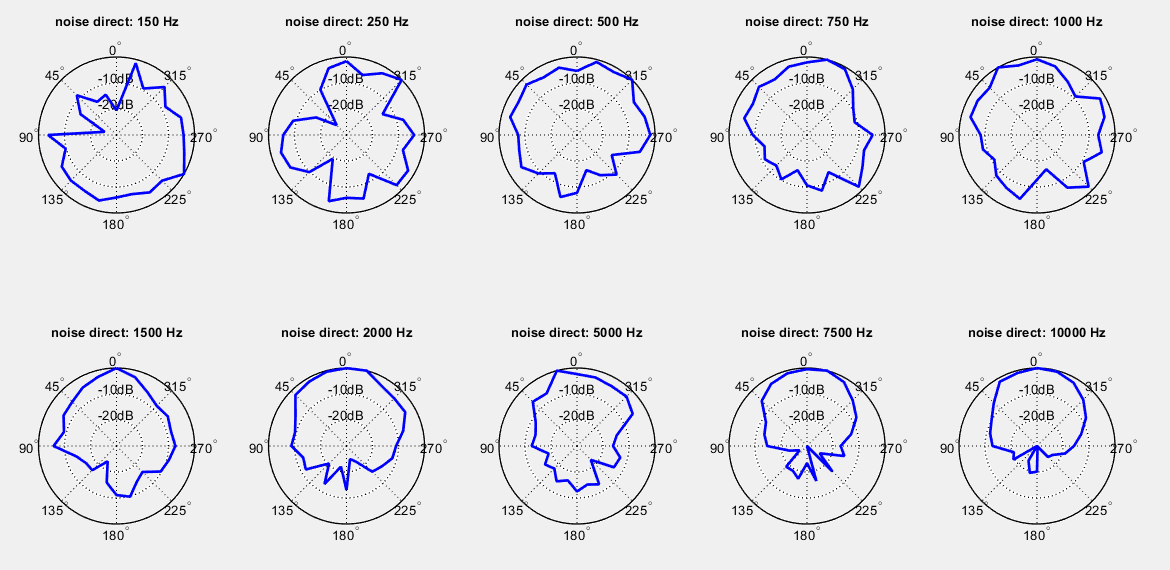
\includegraphics[width=\linewidth]{4a_radiance.png}
		\caption{}
	\end{subfigure}

	\begin{subfigure}{0.85\linewidth}
		\centering
		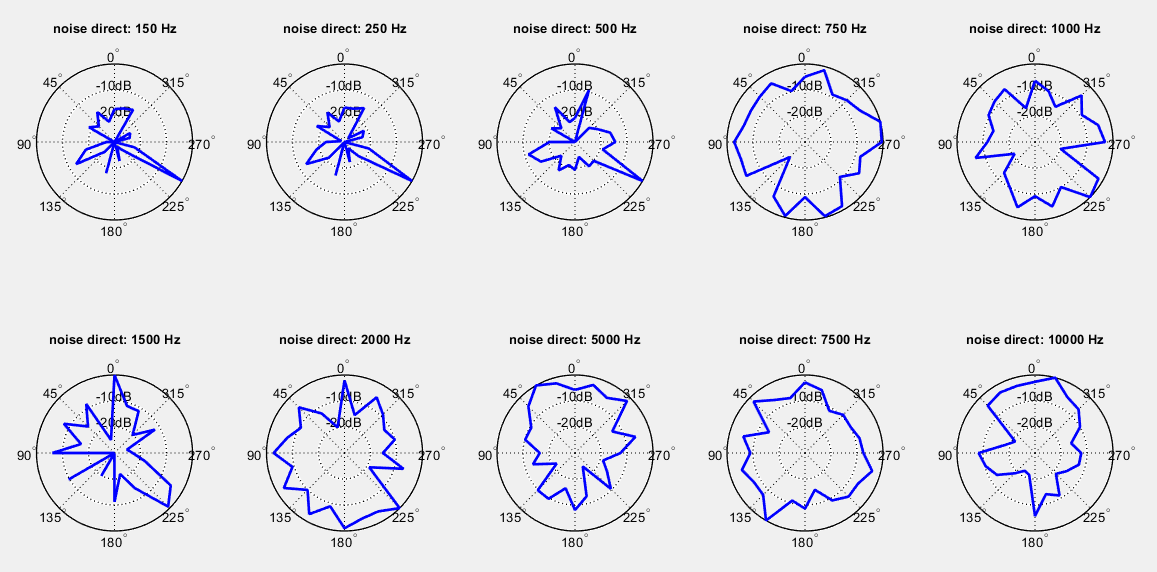
\includegraphics[width=\linewidth]{4a_radiance_120.png}
		\caption{}
	\end{subfigure}
	\caption{Radiance plots for the \textbf{noise signals}. In (a) we used a 701 samples window, while in (b) we used a 241 samples window.}
	\label{fig:noiserad4}
\end{figure}

In both cases the resulting pattern appears rather noisy, which is to be expected since this technique involves quite literally ignoring most of the information collected with the recordings. This suggests why the patterns obtained from the shorter window appear to be worse. Notice however that the noisiest patterns are those in the lower frequency range with the shorter window. This makes perfect sense if we notice that 5 ms is the length of the period of a sinusoid at 200 Hz.

Things get even worse when we move to the sweep signals. Here too we have the same issue with the length of the window. We chose therefore to use the same windows we used before. The radiance plots can be seen in Fig. \ref{fig:sweeprad4}. The main problem here is that, even with the largest window, we are keeping only the first 14 ms of the signal, which doesn't even cover one period of the 50 Hz sinusoid we are starting with. We are therefore losing all of the spectral information, rendering the subsequent computation of the impulse response practically meaningless.

\begin{figure}[h]
	\centering
	\begin{subfigure}{0.85\linewidth}
		\centering
		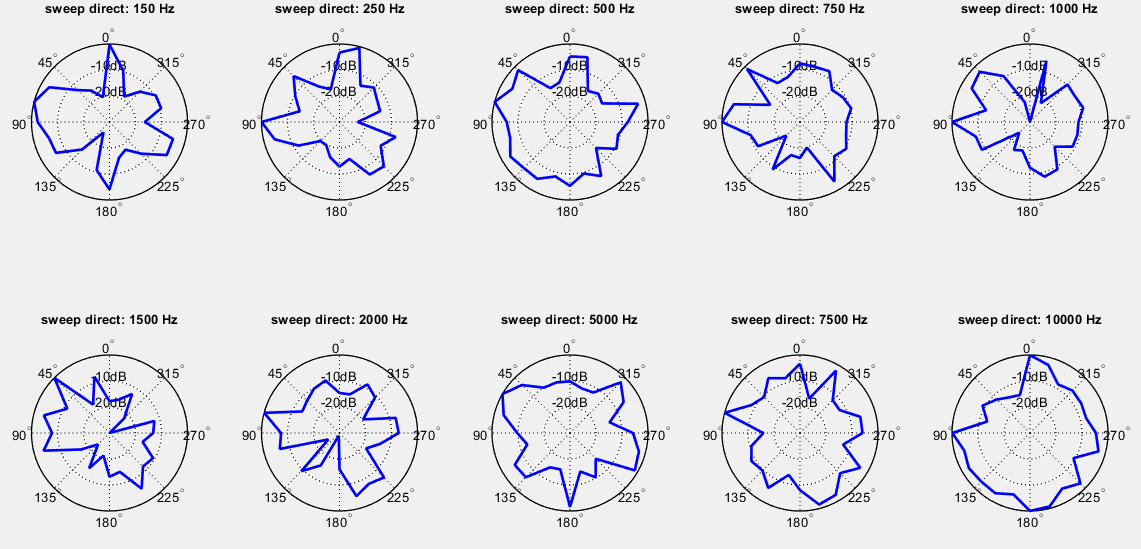
\includegraphics[width=\linewidth]{4b_radiance.png}
		\caption{}
	\end{subfigure}
	
	\begin{subfigure}{0.85\linewidth}
		\centering
		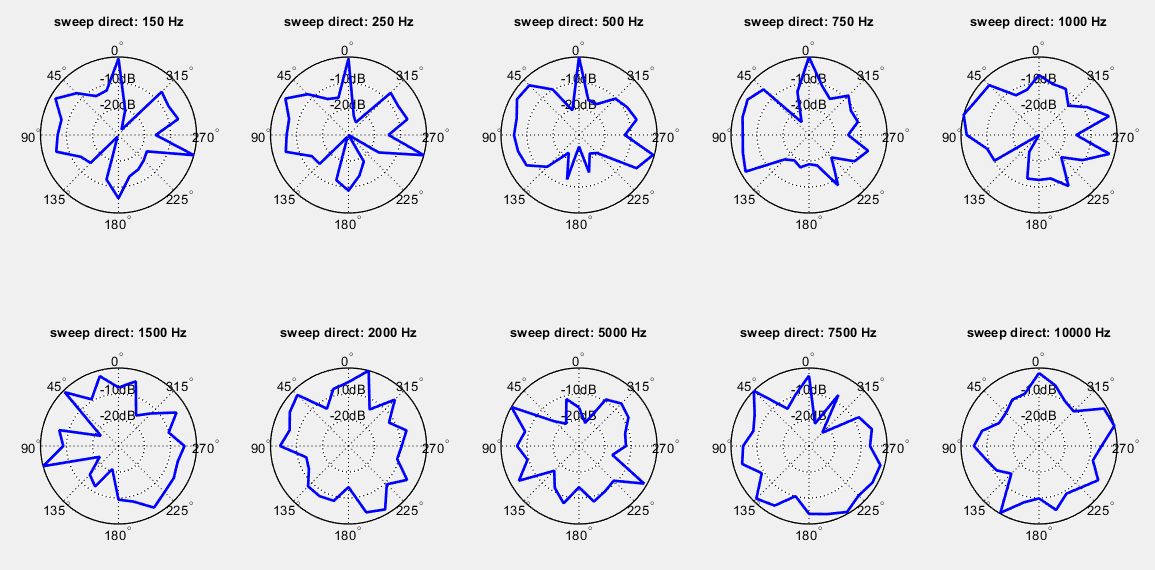
\includegraphics[width=\linewidth]{4b_radiance_120.png}
		\caption{}
	\end{subfigure}
	\caption{Radiance plots for the \textbf{sweep signals}. In (a) we used a 701 samples window, while in (b) we used a 241 samples window.}
	\label{fig:sweeprad4}
\end{figure}

\section{Radiance estimation from the impulse responses}
The scripts we refer to in this section are \verb|exercise5a.m| and \verb|exercise5b.m|. The aim of this section is the same of the previous one, but we set out to use a different (and admittedly more clever) approach, which consists of obtaining the anechoic impulse response by windowing the impulse response itself.
For both kinds of signals, we first used a very short window (101 samples = 2.3 ms), then a larger one that includes the first reflection as well (701 samples = 14.6 ms). The resulting radiation patterns are plotted in Figs. \ref{fig:noiserad5} and \ref{fig:sweeprad5}. We can notice how, when including the first reflection in the window, the radiance around 180° increases: this is because we get the reflected sound from the front of the speaker reflecting off the back wall and reaching the microphone. Furthermore, we also point out that, while with both types of source signal we have a clear  pattern in the higher frequency range, at low frequencies the patterns obtained from the sine sweep appear to be less noisy.

\begin{figure}[h]
	\centering
	\begin{subfigure}{0.85\linewidth}
		\centering
		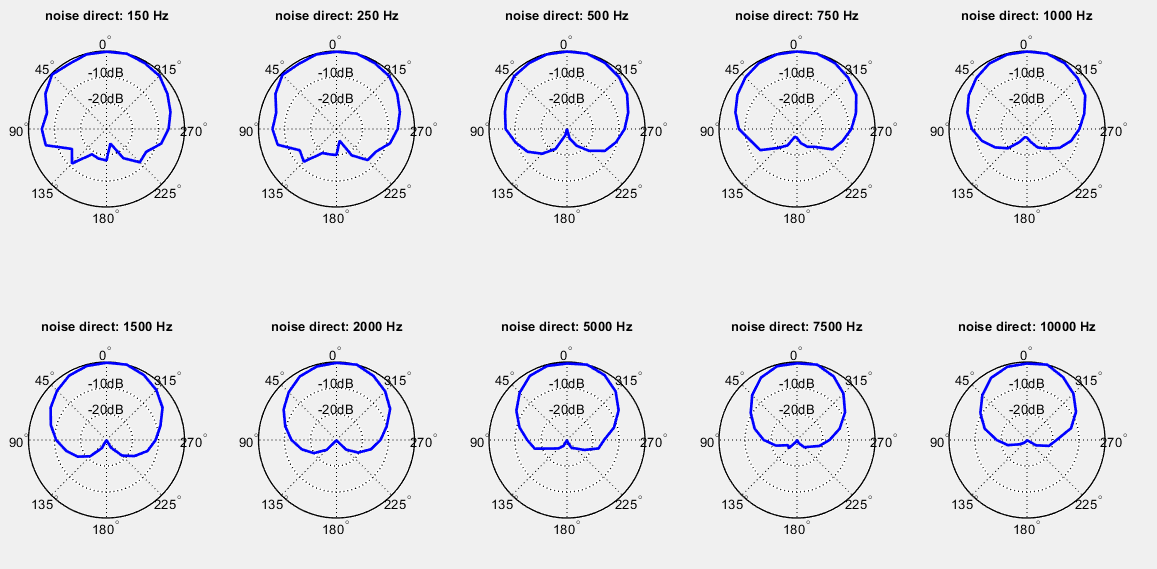
\includegraphics[width=\linewidth]{5a_radiance_50.png}
		\caption{}
	\end{subfigure}
	
	\begin{subfigure}{0.85\linewidth}
		\centering
		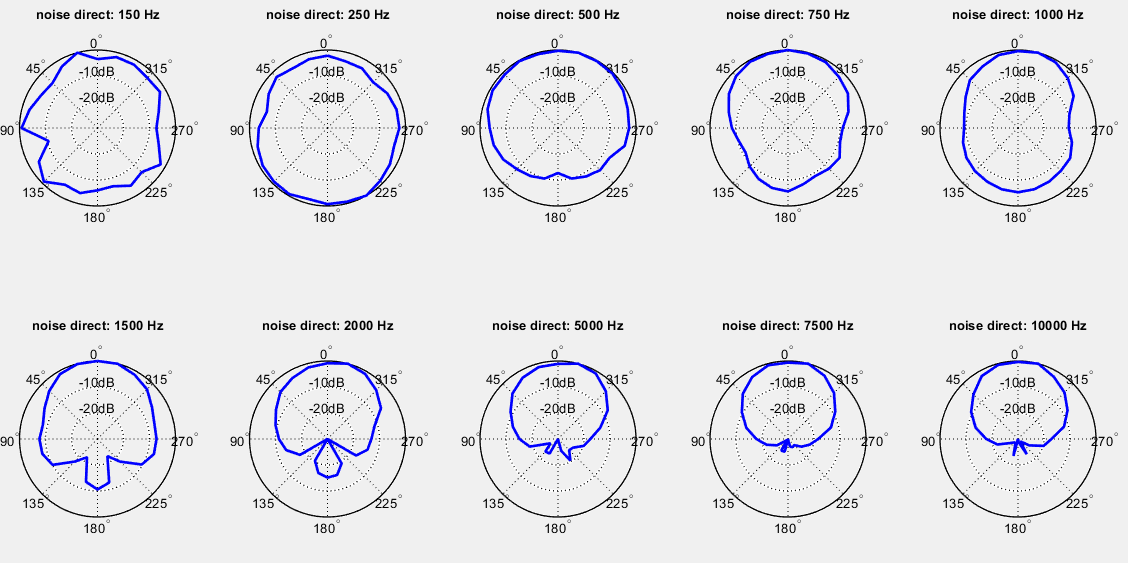
\includegraphics[width=\linewidth]{5a_radiance_350.png}
		\caption{}
	\end{subfigure}
	\caption{Radiance plots for the \textbf{noise signals}. In (a) we used a 101 samples window, while in (b) we used a 701 samples window.}
	\label{fig:noiserad5}
\end{figure}

\begin{figure}[h]
	\centering
	\begin{subfigure}{0.85\linewidth}
		\centering
		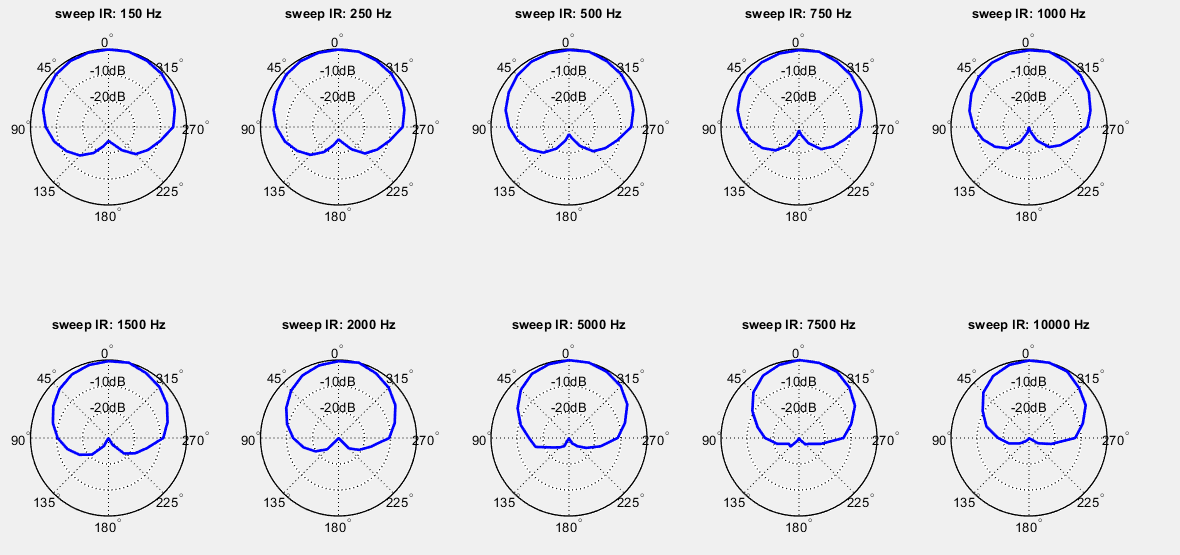
\includegraphics[width=\linewidth]{5b_radiance_50.png}
		\caption{}
	\end{subfigure}
	
	\begin{subfigure}{0.85\linewidth}
		\centering
		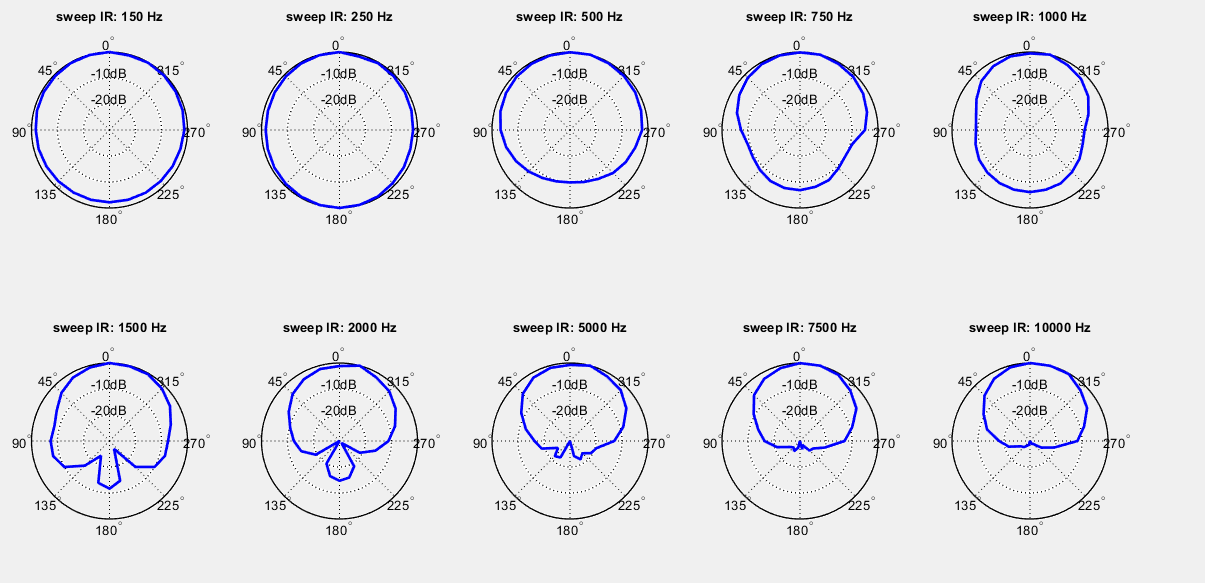
\includegraphics[width=\linewidth]{5b_radiance_350.png}
		\caption{}
	\end{subfigure}
	\caption{Radiance plots for the \textbf{sweep signals}. In (a) we used a 101 samples window, while in (b) we used a 701 samples window.}
	\label{fig:sweeprad5}
\end{figure}



\end{document}